%Antecedentes
\section{Antecedentes}

\begin{frame}[t]
	\vspace{-2mm}
	\begin{block}{¿Clusters solapados?}
	    \begin{center}
   			\only<1>{			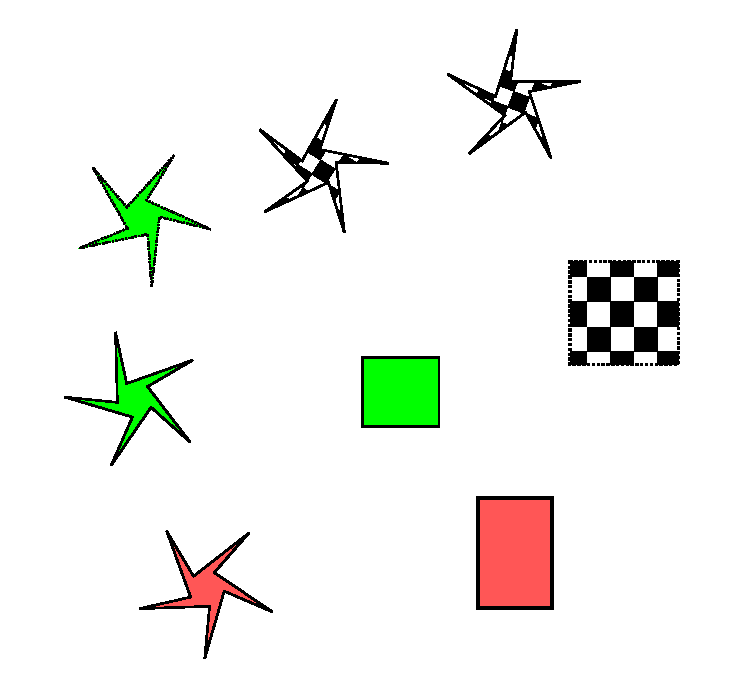
\includegraphics[scale=0.6]{../figs/clustering_bare.pdf}		    }	    
			\only<2>{			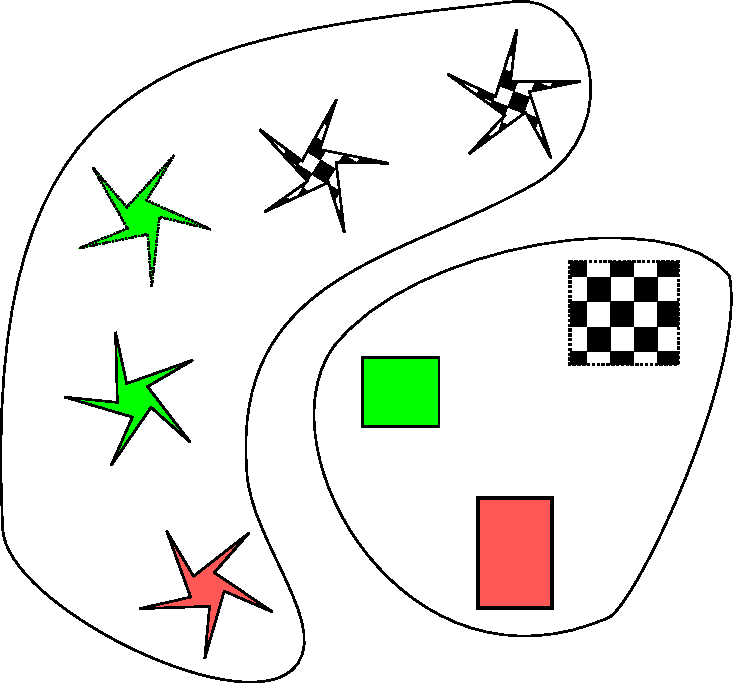
\includegraphics[scale=0.6]{../figs/clustering_shape.pdf}		    }	    
			\only<3>{			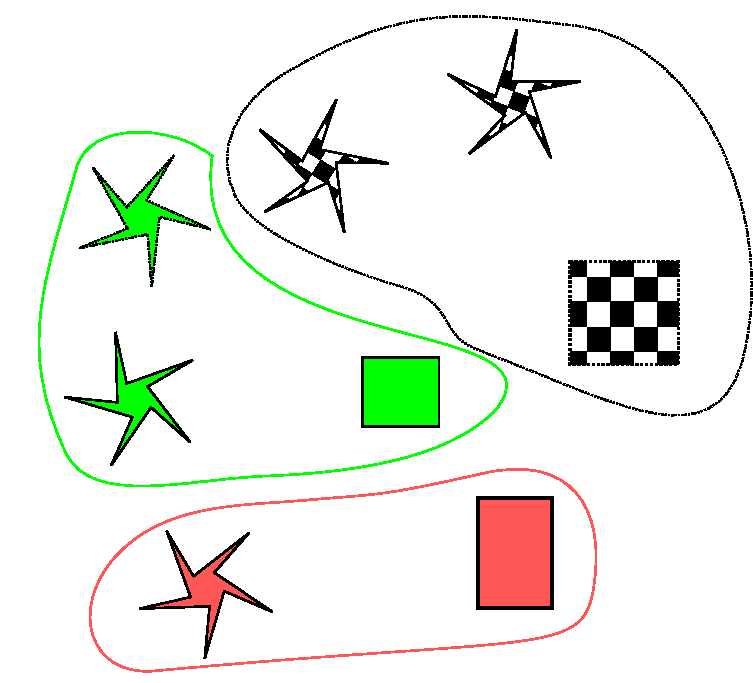
\includegraphics[scale=0.6]{../figs/clustering_fill.pdf}		    }	    
			\only<4->{			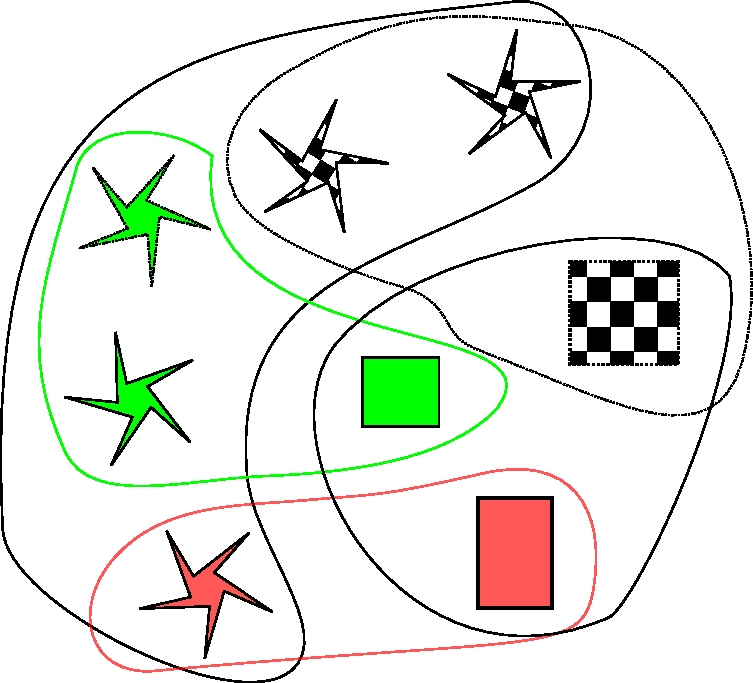
\includegraphics[scale=0.6]{../figs/clustering_all.pdf}		    }	    			
	    \end{center}										
	\end{block}
\end{frame}


\subsection{Medidas de validación externa}
\begin{frame}[t]
	\visible<1->{ 
	\begin{block}{Medidas de validación interna}	
	\end{block}
	}
	\visible<2->{ 
	\begin{block}{Medidas externas de validación}
		Comparan la similitud existente entre un par de soluciones de clustering
		\begin{itemize}
			\item<3-> Conteo de pares de patrones -- Fowlkes--Mallows (FM)
			\item<4-> Correspondencia de conjuntos -- Maximum Match (MM)
			\item<5-> Estadística y teoría de la información -- Normalized Mutual Information (NMI)
		\end{itemize}
	\end{block}
	}
\end{frame}


\subsection{Estado del arte}
\begin{frame}[t]
	\begin{block}{Estado del arte}
		\begin{itemize}
			\item \textit{Zhou et al} (2015) proponen un algoritmo basado en colonia de hormigas para detectar \textbf{comunidades solapadas} en redes de colaboración.
			\item \textit{Liu et al} (2013) presentan un método para caracterizar redes de colaboración compuestas por grupos de \textbf{comunidades} potencialmente \textbf{solapadas}.
			\item \textit{Alvari et al} (2013) ofrecen un framework basado en teoría de juegos para la detección de  \textbf{grupos solapados} en redes sociales.
			\item \textit{Gopalan \& Blei} (2013) proponen un método basado en un modelo Bayesiano para la detección de \textbf{comunidades solapadas} en grandes conjuntos de datos.
		\end{itemize}
	\end{block}
\end{frame}


\subsection{Propuesta}
\begin{frame}[t]
	\begin{block} {Motivación}
		Ninguna de las medidas propuestas hasta el día de hoy es capaz de representar correctamente
		las similitudes entre soluciones de clustering al trabajar con clusters solapados.	
	\end{block}
\vspace{7mm}
\pause
	\begin{block} {Propuesta}
		Nuevo índice de validación externa capaz de trabajar con clusters \textit{solapados}
	\end{block}
\end{frame}
